\documentclass[11pt]{article}
\usepackage[final]{acl}
\usepackage{times}
\usepackage{latexsym}
\usepackage[T1]{fontenc}
\usepackage[utf8]{inputenc}
\usepackage{microtype}
\usepackage{booktabs}
\usepackage{amsmath}
\usepackage{graphicx}
\definecolor{paperblue}{HTML}{003366}
\DeclareCaptionFont{captionlabel}{\color{paperblue}\bfseries}
\captionsetup{labelfont=captionlabel,labelsep=period}
\hypersetup{colorlinks=true,citecolor=paperblue,linkcolor=paperblue,urlcolor=paperblue,
  pdftitle={Does AI Get the Punchline? Learning from Controlled Edits and Testing Transfer to Natural Memes}}
\title{\textcolor{paperblue}{Does AI Get the Punchline?}\\
Learning from Controlled Edits and Testing Transfer to Natural Memes}
\author{MemeVLM Project Team}
\setcounter{dbltopnumber}{3}
\renewcommand{\dbltopfraction}{.86}
% Generated from the frozen full-study aggregate.
\newcommand{\PrimaryBase}{53.55}
\newcommand{\PrimaryBilingual}{54.82}
\newcommand{\PrimaryChinese}{53.92}
\newcommand{\PrimaryContrast}{$+1.27$}
\newcommand{\PrimaryInterval}{$[{-}1.14, 3.58]$}
\newcommand{\PrimaryValidSummary}{816/816 valid answers}
\newcommand{\SyntheticBase}{37.5}
\newcommand{\SyntheticBilingual}{92.7}
\newcommand{\SyntheticChinese}{57.3}
\newcommand{\SyntheticContrast}{$+35.42$}
\newcommand{\SyntheticInterval}{$[21.88, 50.00]$}
\newcommand{\SyntheticDiagnosticSummary}{each arm had 96/96 valid answers and 96/96 correct cues}
\newcommand{\TargetBase}{20/32}
\newcommand{\TargetBilingual}{31--32 of 32}
\newcommand{\TargetChinese}{25/32}

\begin{document}
\raggedbottom
\maketitle
\begin{abstract}
Does a model revise a meme's interpretation when the visual evidence changes? We compare mixed-corpus and replay LoRA recipes on Qwen3-VL-4B with the same update budget and three paired seeds. Across 32 authored edit families, mean strict accuracy is \SyntheticBilingual\% with the mixed corpus, \SyntheticChinese\% with replay and \SyntheticBase\% with the frozen base. Every model identifies the cue in all 96 images. Relation choices account for the accuracy gap. On 816 MemeQA questions across 134 natural images outside an earlier pilot, the mixed-corpus recipe gains 0.90 percentage points over replay (95\% image-bootstrap interval $[-1.18,2.99]$) and \PrimaryContrast\ points over the frozen base (\PrimaryInterval). Both intervals include zero. In a separate MemeBench edit test, frozen 4B and 8B each pass 5/10 complete triples.
\IfFileExists{coverage-results.tex}{A post-hoc MemeBench audit finds higher reasoning coverage with images than with OCR. The relative gains in knowledge and reasoning from hints remain uncertain.}{}
\end{abstract}

\section{Introduction}

A fitness watch classifies its wearer's afternoon as active. If the wearer spent three hours clapping, the joke is that the device mistook applause for exercise. Replacing \emph{clapping} with \emph{walking} removes that mismatch. A model can read the new word correctly and still repeat the old interpretation. A test of interpretation should therefore check both the visible cue and the relation the model attributes to it.

Literal description and intended meaning are separate annotation targets in MemeCap \citep{hwang2023memecap}. MemeBench further separates visual details, identity, background knowledge, and reasoning in explanations \citep{wang2026meme}. MER-Bench studies how editing a meme can change its emotional appraisal while preserving the original situation \citep{nie2026merbench}. Together these tasks motivate two complementary edits. One changes evidence that warrants a new reading. The other changes an incidental detail that should leave the interpretation intact.

\paragraph{Study design.}
We use a pretrained Qwen3-VL checkpoint and standard LoRA. We author edit families, implement strict family scoring, and compare mixed-corpus training with replay under a matched budget. The same models take the authored edit test and answer native MemeQA questions outside an earlier pilot \citep{nguyen2025memeqa}. The outcomes are strict family accuracy and pooled question accuracy. A separate MemeBench study assesses edits and explanation coverage with frozen models.

\section{Data and adaptation}

\paragraph{Authored edit families.}
We write the scenarios and choices in English and render the memes as comics, status screens, chats and posters. Each of eight mechanisms contributes 21 training, five validation and four test families, giving 168, 40 and 32 families, respectively. Each family shares its setup and answer choices across an original, a target edit and a sham. A target edit changes the relation supported by the image. A sham changes a corner mark while preserving the original cue and relation. Each training or validation family supplies one free explanation and three cue--relation answers. Figure~\ref{fig:examples} shows one held-out family.

\begin{figure*}[t]
\centering
\newcommand{\watchpanel}[2]{\begin{minipage}[t]{.316\textwidth}\centering
 {\small\bfseries\textcolor{paperblue}{#1}}\\[3pt]
 \includegraphics[width=.91\linewidth]{../assets/watch-#2.png}
 \end{minipage}}
\watchpanel{Original}{original}\hfill\watchpanel{Target edit}{edited}\hfill\watchpanel{Sham edit}{sham}
\caption{An illustrative edit family. The original watch counts clapping as exercise. The target replaces clapping with walking in both the text and pictogram, making the activity label reasonable. The sham changes a corner mark. In evaluation, the base detects the target cue and retains the original interpretation. The seed-42 mixed-corpus adapter changes its relation judgment. Both preserve the original interpretation on the sham.}
\label{fig:examples}
\end{figure*}

\paragraph{Mixed corpus and replay.}
The mixed corpus contains 672 English rows on 504 images and 98 Chinese rows on 98 images. The shared training pool includes two MemeXGen examples \citep{zhao2026memexgen}. The common validation set has 193 rows on 153 images (160 English rows and 33 Chinese), with one additional MemeXGen example. Split checks cover family membership and exact decoded-image overlap.

Both recipes use 770 row exposures per epoch (Figure~\ref{fig:training}). Mixed-corpus training visits each row once. Replay (Chinese replay) repeats each of the 98 shared rows seven times and presents a fixed subset of 84 once more.

\begin{figure*}[t]
\centering
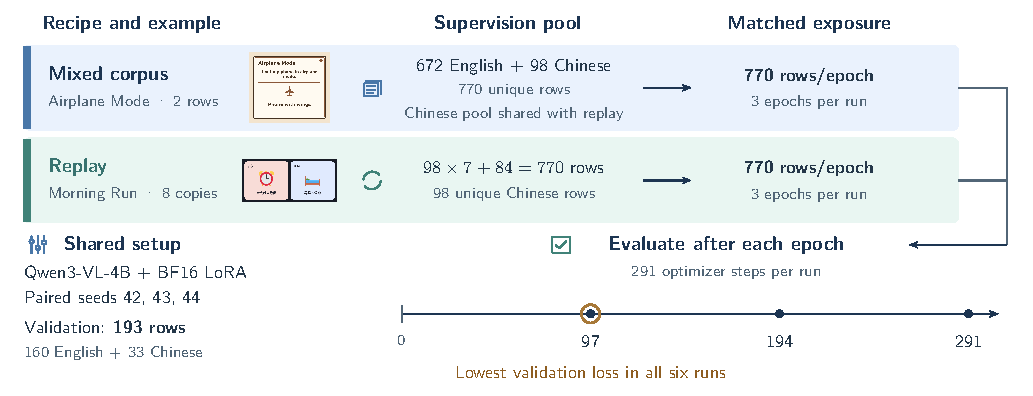
\includegraphics[width=.95\textwidth]{../figures/matched-training.pdf}
\caption{Training exposure under each recipe. Airplane Mode provides two distinct supervision rows. Morning Run provides one row and appears eight times in each replay epoch. Both recipes use the same validation examples, checkpoint schedule and optimization budget.}
\label{fig:training}
\end{figure*}

\paragraph{Model and optimization.}
The fixed comparator is Qwen3-VL-4B-Instruct \citep{bai2025qwen3vl}. Its vision encoder extracts patch features. A patch merger maps those features to the language model's input space, and three intermediate visual features enter the early language blocks through DeepStack. LoRA updates the attention and feed-forward projections in all 36 language blocks ($r=8$, $\alpha=16$) \citep{hu2022lora}. The vision encoder, visual mergers and base language weights remain frozen (Figure~\ref{fig:architecture}).

\begin{figure*}[t]
\centering
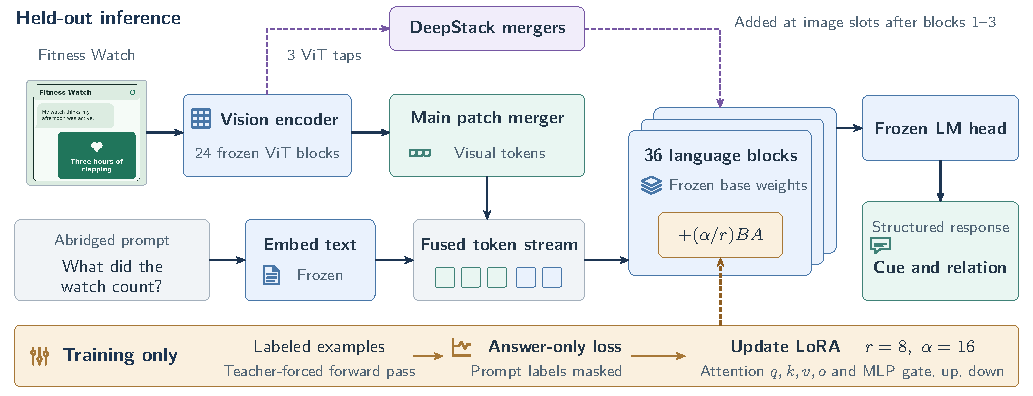
\includegraphics[width=.95\textwidth]{../figures/qwen3vl-lora.pdf}
\caption{Visual and textual inputs to the adapted Qwen3-VL model. The upper path traces one held-out choice. The lower path shows how the answer-token loss updates the low-rank factors in language-layer attention and feed-forward projections.}
\label{fig:architecture}
\end{figure*}

Both recipes use completion-only cross-entropy, BF16, a 2{,}048-token limit and a 262{,}144-pixel cap. AdamW uses a learning rate of $10^{-4}$, cosine decay and 10\% warmup. Each run completes three epochs (291 optimizer steps) with batch size one and eight accumulated minibatches per update. We pair training and data-order seeds 42, 43 and 44 across recipes. Each run selects the checkpoint with the lowest loss on the common validation set among steps 97, 194 and 291.

\section{Evaluation}

\paragraph{Controlled edits.}
All seven model arms use identical prompts within each evaluation, greedy decoding and a 512-token cap. For every synthetic image the model returns a cue judgment, a relation choice and a nonempty explanation. The scorer maps the displayed choice to a semantic relation and checks it against the variant-specific key. Let $J_{fv}$ indicate that the response for family $f$ and variant $v$ is valid and both judgments are correct. Strict success requires
\[
S_f = J_{f,\mathrm{original}} J_{f,\mathrm{target}} J_{f,\mathrm{sham}} = 1.
\]
The exact score uses the cue and relation choices. A nonempty explanation satisfies the prose requirement. The same 32 held-out families appeared in the initial comparison of the base and seed-42 mixed-corpus adapter.

\paragraph{Natural memes.}
MemeQA's $\mathrm{None}^{-}$ split omits the \emph{none of the above} choice and filters out questions answered correctly by a text-only model in the original study \citep{nguyen2025memeqa}. We take all 1{,}027 eligible single-answer, four-option English test questions on 166 images and preserve the question and choice text. A fixed permutation balances correct answer positions in the primary cohort (204 per letter). Excluding all 32 pilot images leaves 816 questions on 134 images for the primary analysis. The full eligible set serves as a sensitivity check. Exact decoded RGB comparison found zero matches against 956 project images.

We measure pooled question accuracy on this subset. The published MemeQA overall score macro-averages across question types and includes multi-answer tasks. Our primary cohort comprises 448 intent-completion, 263 derivation-completion, 67 conditional-action and 38 intent-identification questions. Thus 87.1\% of these questions ask the model to fill in a missing part of a statement.

\paragraph{Uncertainty.}
We average the three fitted seeds per recipe and report their sample standard deviation separately. For paired contrasts we draw 10{,}000 bootstrap samples of synthetic families or natural images with replacement, retaining all arms and all questions within a sampled cluster. On MemeQA each draw pools correct answers over its sampled questions. Percentile intervals quantify variation across evaluation clusters, conditional on the fitted models.

\paragraph{Fixed-model edits and reference coverage.}
We select 60 Chinese MemeBench families (20 development, 40 test) and reuse their OCR and checklists for visual detail, identity, knowledge and reasoning (V/I/K/R). We curate hints and author target and sham edits for 15 families (5 development, 10 test). Frozen 4B and 8B explain the original from image, OCR, or image with a factual hint using greedy decoding and a 512-token cap. Two AI-generated reviews of ten development explanations inform the scoring setup. InternVL3-9B sees the original, public reference, checklist and anonymized explanation, and labels checklist items within 768 tokens \citep{opengvlab2025internvl3}. The frozen rule requires the full checklist, valid JSON (bare or fenced) and one or two distinct in-range span IDs per covered item. IDs resolve to literal candidate text. Paired coverage uses valid scores under both inputs, out of 35 families with transcripts for OCR and all 40 for hints. The edit task uses exact cue and relation scoring and repeats each test original with reordered choices.

% Generated from the frozen full-study aggregate.
\begin{table*}[t]
\centering
\small
\begin{tabular}{@{}lrrr@{}}
\toprule
Arm & Synthetic strict triples & MemeQA primary & MemeQA all-eligible\\
\midrule
Frozen base & 37.5 & 53.55 & 53.75\\
\midrule
Mixed corpus, seed 42 & 93.8 & 54.41 & 54.14\\
Mixed corpus, seed 43 & 93.8 & 55.39 & 55.01\\
Mixed corpus, seed 44 & 90.6 & 54.66 & 54.72\\
Mixed corpus, mean $\pm$ SD & $92.7 \pm 1.8$ & $54.82 \pm 0.51$ & $54.63 \pm 0.45$\\
\midrule
Replay, seed 42 & 59.4 & 54.17 & 54.43\\
Replay, seed 43 & 59.4 & 53.92 & 54.24\\
Replay, seed 44 & 53.1 & 53.68 & 54.04\\
Replay, mean $\pm$ SD & $57.3 \pm 3.6$ & $53.92 \pm 0.25$ & $54.24 \pm 0.19$\\
\bottomrule
\end{tabular}
\caption{Accuracy (\%) by arm. Synthetic scoring uses 32 families, with all three variants required for a pass. MemeQA primary uses 816 questions on 134 images outside the pilot. All-eligible sensitivity uses 1{,}027 questions on 166 images. SD is the sample standard deviation across three seeds.}
\label{tab:full-scores}
\end{table*}

\begin{table*}[t]
\centering
\small
\begin{tabular}{@{}lrrr@{}}
\toprule
Cohort & Mixed corpus $-$ base & Replay $-$ base & Mixed corpus $-$ replay\\
\midrule
Synthetic strict triples & $+55.21\;[38.54, 71.88]$ & $+19.79\;[5.21, 34.38]$ & $+35.42\;[21.88, 50.00]$\\
MemeQA primary & $+1.27\;[{-}1.14, 3.58]$ & $+0.37\;[{-}1.19, 1.91]$ & $+0.90\;[{-}1.18, 2.99]$\\
MemeQA all-eligible & $+0.88\;[{-}1.15, 2.89]$ & $+0.49\;[{-}0.86, 1.82]$ & $+0.39\;[{-}1.43, 2.21]$\\
\bottomrule
\end{tabular}
\caption{Paired differences in percentage points with 95\% percentile bootstrap intervals. Each draw resamples synthetic families or natural images, together with all their questions and arms. Intervals condition on the fitted adapters.}
\label{tab:full-contrasts}
\end{table*}


\paragraph{Teammate audit.}
After judge freeze, two teammates each rated 120 development and 240 held-out explanations. Forms hide model, condition and judge labels and remove input markers in 80 test responses. Coverage is the fraction marked covered per dimension. From the submitted scores we compare item labels and paired family means (95\% intervals, 10{,}000 family resamples). The fixed audit includes ten development and twenty test cases.

\section{Results}

\paragraph{Training and checkpoint selection.}
Training loss falls in each run, yet validation loss is lowest at the first measured checkpoint in all six (Figure~\ref{fig:loss}). Between steps 97 and 291, mean validation loss rises from $0.713$ to $1.015$ for the mixed corpus and from $2.903$ to $3.068$ for replay. We use the step-97 adapters for both held-out tests. Validation loss uses a shared set with 193 rows. \mbox{Of those, 160 are authored examples.}

\begin{figure*}[t]
\centering
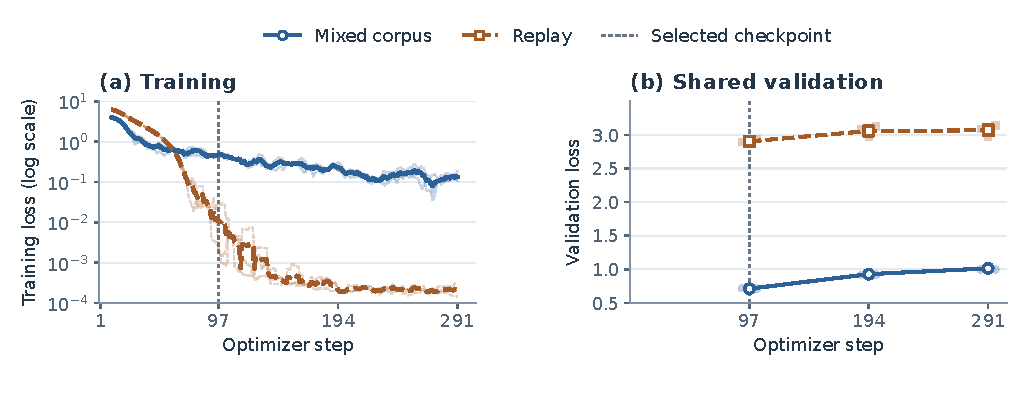
\includegraphics[width=.91\textwidth]{../figures/training-diagnostics.pdf}
\caption{Training and validation loss over the six adaptation runs. Training curves use trailing ten-step means on a log scale. The three validation checkpoints use the same 193 rows. Thin curves or small markers denote individual seeds. Bold curves and error bars denote means and one sample standard deviation.}
\label{fig:loss}
\end{figure*}

\paragraph{Relation choices account for the controlled-task gain.}
The mixed-corpus adapters pass 29 or 30 of 32 families per seed, compared with 17--19 for replay and 12 for the frozen base (Table~\ref{tab:full-scores}). The mixed-corpus advantage over replay is \SyntheticContrast\ percentage points (95\% interval \SyntheticInterval, Table~\ref{tab:full-contrasts}). Each arm produces 96/96 valid responses and identifies the cue in all 96 images. On target edits, the base selects the correct cue and relation on \TargetBase, replay on 25/32 in each seed, and the mixed-corpus adapters on \TargetBilingual. The Fitness Watch error shows how recognizing a cue can coexist with an incorrect interpretation (Figure~\ref{fig:examples}).

\paragraph{Gains on natural questions are small.}
On the primary MemeQA cohort the base solves 437/816 questions (\PrimaryBase\%). The mixed-corpus adapters solve 444, 452 and 446 (\PrimaryBilingual\% mean). Replay solves 442, 440 and 438 (\PrimaryChinese\% mean). All seven arms return 816 valid choices. Relative to same-seed replay, the mixed-corpus adapters change roughly as many answers from correct to wrong as from wrong to correct (Figure~\ref{fig:memeqa-transitions}). The difference is $+0.90$ points ($[-1.18,2.99]$) over replay and \PrimaryContrast\ points over the base (\PrimaryInterval). Including the pilot images gives a similar result.

\begin{figure*}[t]
\centering
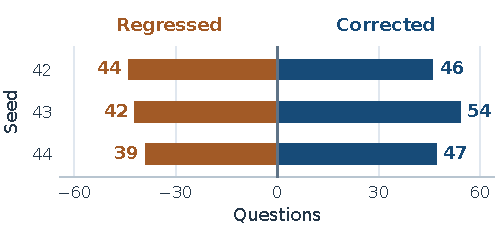
\includegraphics[width=.55\linewidth]{../figures/memeqa-transitions.pdf}
\caption{Paired changes on natural memes. Relative to same-seed replay, mixed-corpus adaptation corrects errors and introduces new ones across 816 identical questions per seed.}
\label{fig:memeqa-transitions}
\end{figure*}

\begin{figure*}[t]
\centering
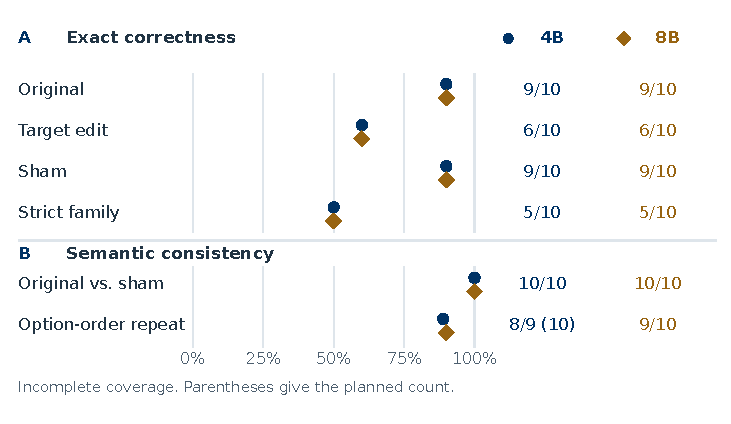
\includegraphics[width=.76\textwidth,height=56mm,keepaspectratio]{../figures/rq3-test.pdf}
\caption{Frozen Qwen3-VL models on ten held-out MemeBench edit families. Exact correctness requires both the cue and relation to match the key. Semantic consistency compares the relation IDs. Option-order agreement counts valid original--repeat pairs. Parentheses show the planned denominator.}
\label{fig:chinese-edits}
\end{figure*}

\paragraph{Fixed-model edit diagnostic.}
On ten test families, 4B and 8B each detect the cue in all 30 images. Each selects the correct relation on 9/10 originals, 6/10 targets, and 9/10 shams (Figure~\ref{fig:chinese-edits}). Within each model, target edits reduce joint accuracy by 30 percentage points (95\% paired family-bootstrap interval $[-70,+10]$). Both models pass 5/10 complete triples (95\% interval $[20,80]\%$). Original--sham semantic agreement is 10/10, including one incorrect original interpretation per model. After option reordering, agreement is 8/9 for 4B and 9/10 for 8B. One 4B repeat has an invalid format. Both models pass 2/5 development triples.

\IfFileExists{coverage-results.tex}{%
  \paragraph{Automatic reference coverage.}
  The frozen rule accepts 91/240 held-out judgments. The 149 rejections reflect the citation-count rule (105), malformed JSON (27), the token cap (12), or missing checklist items (5). Each paired contrast uses at most five families. The 4B hint comparison has zero valid pairs.
  \IfFileExists{coverage-replay-results.tex}{%
    Replay removes the citation cap and accepts 188/240 stored judgments. On replay pairs, image inputs yield higher reasoning coverage than OCR. Hint gains favor knowledge over reasoning in both models.
    \IfFileExists{../figures/reference-coverage-replay.pdf}{%
      Figure~\ref{fig:replay-coverage} shows the paired coverage contrasts.
      \begin{figure*}[t]
      \centering
      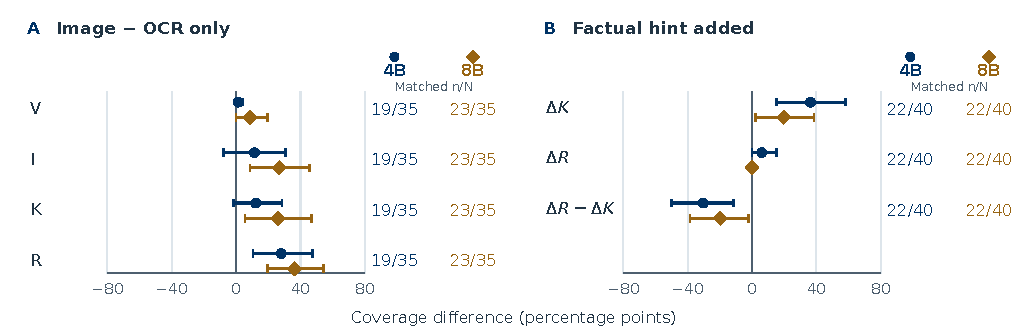
\includegraphics[width=.96\textwidth,height=50mm,keepaspectratio]{../figures/reference-coverage-replay.pdf}
      \caption{Post-hoc replay of MemeBench coverage judgments without the citation cap. The OCR panel reports matched families out of 35 with transcripts and the hint panel reports matched families out of 40 planned. Points show mean within-family differences with paired 95\% family-bootstrap intervals. $\Delta R-\Delta K$ uses families scorable for both dimensions under both inputs.}
      \label{fig:replay-coverage}
      \end{figure*}
    }{}
  }{\IfFileExists{../figures/reference-coverage-test.pdf}{%
    Figure~\ref{fig:chinese-coverage} shows the paired estimates and intervals.
    \begin{figure*}[t]
    \centering
    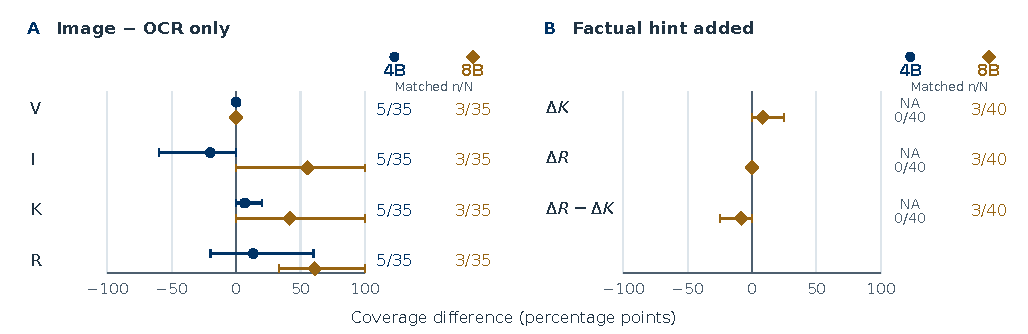
\includegraphics[width=.96\textwidth,height=50mm,keepaspectratio]{../figures/reference-coverage-test.pdf}
    \caption{Exploratory AI-assisted scores for MemeBench explanations. The image--OCR comparison reports matched families out of 35 with source transcripts. The factual-hint comparison reports matched families out of 40 planned. Points are mean within-family differences and bars are paired 95\% family-bootstrap intervals. The reasoning-minus-knowledge contrast uses families scorable on both dimensions under both inputs.}
    \label{fig:chinese-coverage}
    \end{figure*}
  }{}}
}{}

\IfFileExists{coverage-results.tex}{%
\paragraph{Audit of explanation scoring.}
Teammates agree on 4{,}354/4{,}386 checklist items, including 2{,}929/2{,}952 in test. The sheets differ on 45 fields across 17 explanations. Both credit an unstated release year and distributor in one answer and mark identical abstentions as grounded. Table~\ref{tab:human-audit} shows judge agreement on each rule's available subset. Replay preserves every verdict on the 91 shared explanations. The judge uses full answers and the teammates use the blinded display.

\smallskip\noindent\begin{minipage}{\columnwidth}
\centering
\small
\setlength{\tabcolsep}{3.5pt}
\begin{tabular}{lrrrr}
\toprule
Rule & Valid & Fixed test & R1 items & R2 items \\
\midrule
Frozen & 91/240 & 11/20 & 560/1{,}110 & 560/1{,}110 \\
Replay & 188/240 & 17/20 & 1{,}441/2{,}297 & 1{,}440/2{,}297 \\
\bottomrule
\end{tabular}
\captionof{table}{Valid test judgments and exact item agreement with each teammate. Fixed test denotes the proposal's 20-case subset.}
\label{tab:human-audit}
\end{minipage}\par\smallskip

\paragraph{RQ1, image versus OCR.}
Across the 35 transcript-eligible families, reasoning gains are $+57.1$ points for both 4B ratings and $+76.7$/$+77.6$ for 8B (R1/R2). All four coverage dimensions improve for both models and raters, with 95\% intervals above zero.

\paragraph{RQ2, factual hints.}
Across 40 families, knowledge gains are $+26.0$/$+24.2$ points for 4B and $+12.9$/$+16.0$ for 8B. Reasoning gains are $+29.6$/$+27.1$ and $+11.2$/$+12.1$, respectively. All four intervals for the reasoning-minus-knowledge gain include zero. Gains shrink after excluding 13 families flagged by either rater for direct hint leakage. Only 4B reasoning retains intervals above zero. The automatic replay's larger knowledge gains describe its matched subset. In an AI-assisted sensitivity analysis with 62 proposed test checklist edits, hint knowledge gains drop by $1.9$--$2.5$ points and the conclusions for both questions hold.
}{}

\section{Discussion}

The authored test shares its renderer, mechanism categories and answer style with training. Text changes alongside pictograms. At matched optimizer steps and row exposures, we estimate the effect of the full recipe. Example diversity, language mix, task formats and token composition vary together.

On MemeQA, new errors offset many corrected answers. Both paired intervals include zero, leaving transfer to this predominantly completion-based task uncertain.

The earlier 2B pilot used the same ten MemeBench test triples. The frozen 4B and 8B results diagnose these fixed examples. Pretraining exposure to the public memes is unknown.

\section*{Acknowledgments}
Generative AI assisted scenario drafting, implementation and writing.

\IfFileExists{coverage-results.tex}{\clearpage}{\newpage}
\bibliography{references}
\end{document}
